\section{数据预处理}
\label{sec:data}

\subsection{数据结构与状态变量统一}
表单1、表单2和表单3分别对应文物、已分类采样点及未知文物三个层级。
前者含58件已分类文物的类型、纹饰、颜色和整体表面风化信息；表单2含69个采样点的14种化学成分；表单3含A1--A8共8个未知样品。
因此，问题一至四均以采样点层的化学成分建模，文物编号仅用于关联属性与分组交叉验证；不以文物代表成分代替采样点数据。
对采样点状态逐行按完整采样点名称判定：含``未风化点''者归入未风化组，含``严重风化点''者归入风化组并保留严重标签，其余为普通点；普通点的二元风化状态才关联表单1属性，避免把同一文物的普通部位和特殊部位混为一类。

\subsection{有效性检验与未检出成分}
记第\(i\)件文物第\(r\)个采样点第\(j\)种成分的原始比例为\(x_{irj}\)，其14种成分和为
\begin{equation}
    S_{ir}=\sum_{j=1}^{14}x_{irj}.
    \label{eq:composition-sum}
\end{equation}
按题意仅保留\(85\leq S_{ir}\leq105\)的化学成分记录。表\ref{tab:data-cleaning}表明，15、17号的成分和分别为79.47\%和71.89\%，故只剔除其化学成分记录；其在表单1中的类型、纹饰、颜色与风化属性仍予保留。表单3的8条记录均通过该检验。

\begin{table}[H]
    \centering
    \caption{数据清洗结果汇总}
    \label{tab:data-cleaning}
    \small
    \begin{tabular}{lrrrr}
        \toprule
        数据对象 & 原始记录数 & 有效记录数 & 剔除记录 & 未检出成分单元格 \\
        \midrule
        已分类文物（表单1） & 58 & 58 & 0 & -- \\
        已分类采样点（表单2） & 69 & 67 & 2（15、17号） & 317/938（33.80\%） \\
        未知样品（表单3） & 8 & 8 & 0 & 按同一规则处理 \\
        \bottomrule
    \end{tabular}
\end{table}

附件中的空白表示未检出，不视为随机缺失：求和、频数和原始比例统计均按0计，不对化学成分作均值或热卡填补。图\ref{fig:data-diagnostics}左侧显示了筛选阈值与两条无效记录，右侧给出有效点各成分的未检出率，为后续对数比变换提供依据。

\begin{figure}[H]
    \centering
    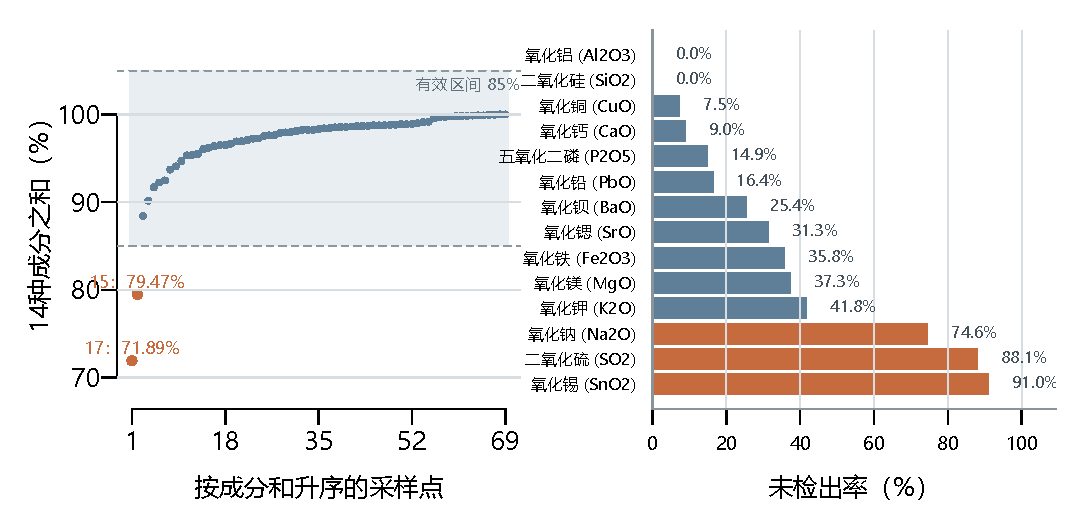
\includegraphics[width=0.96\textwidth]{figures/data_preprocess_diagnostics.pdf}
    \caption{成分和有效性与各成分未检出率组合诊断}
    \label{fig:data-diagnostics}
\end{figure}

\subsection{代表成分与颜色热卡填补}
仅为补全4件颜色缺失文物，按文物编号构造代表成分：单一采样点直接采用；两个普通部位取14种成分的算术平均；普通部位与严重风化点按\(1:2\)加权；普通部位与未风化点并存时采用普通部位；只有未风化点时取其均值。上述普通、未风化和严重风化状态均由完整采样点名称逐行判定；无效的15、17号成分不参与代表成分和供体距离计算。

对代表成分依次闭合、近零替换并作CLR变换，在CLR空间以欧氏距离计算Aitchison距离。供体限定为玻璃类型、纹饰均相同且颜色已知的文物，取最近5个供体按距离倒数投票；若获胜颜色票重占比不足50\%，则回退至同玻璃类型颜色众数。结果见表\ref{tab:color-imputation}；40号因票重不足而回退，且对近零参数较敏感，故问题一另以“使用填充值/排除4件缺色文物”作对照分析。

\begin{table}[H]
    \centering
    \caption{缺失颜色的文物级填补结果（\(\delta=0.02\%\)）}
    \label{tab:color-imputation}
    \small
    \begin{tabular}{ccc}
        \toprule
        文物编号 & 最终颜色 & 处理方式 \\
        \midrule
        19 & 黑 & 热卡填补 \\
        40 & 浅蓝 & 票重不足50\%，同类型众数回退 \\
        48 & 浅蓝 & 热卡填补 \\
        58 & 浅蓝 & 热卡填补 \\
        \bottomrule
    \end{tabular}
\end{table}

\subsection{闭合、近零替换与CLR变换}
为消除记录总量偏离100\%造成的不可比性，先对每个有效采样点闭合：
\begin{equation}
    c_{irj}=100\frac{x_{irj}}{S_{ir}}.
    \label{eq:closure}
\end{equation}
有效训练数据的最小正成分为0.04\%，取其一半\(\delta=0.02\%\)。若一行有\(k\)个零值，则每个零替换为\(\delta\)，其余正成分统一乘以\((100-k\delta)/100\)，从而仍保持行和为100\%。在\(\delta=0.01\%,0.02\%,0.04\%\)下重复诊断，均未产生新增剔除点；相对\(0.02\%\)基准，供体集合分别有3、0、4处变化。颜色及供体对近零参数的完整变化由敏感性工作表记录，因此将颜色填补作为不确定性来源在问题一中作“保留填充值/剔除缺色文物”的对照，而不将其当作确定观测。

随后以中心对数比变换进入成分分析空间：
\begin{equation}
    z_{irj}=\ln\!\left(\frac{c_{irj}^{+}}
    {\left(\prod_{j=1}^{14}c_{irj}^{+}\right)^{1/14}}\right).
    \label{eq:clr}
\end{equation}
需要统一尺度的分类或聚类模型再取\(u_{irj}=(z_{irj}-\mu_j)/\sigma_j\)。\(\mu_j,\sigma_j\)仅由已分类训练集估计，表单3只套用表单2参数；交叉验证时以文物编号分组，并在每一训练折重新估计参数，以避免同一文物泄漏及标准化泄漏。图\ref{fig:data-flow}概括了该处理链。

\begin{figure}[H]
    \centering
    \begin{tikzpicture}[
        >=Latex,
        data/.style={draw=black!55, rounded corners=2pt, fill=blue!5, align=center, text width=3.25cm, minimum height=1.35cm, font=\small},
        process/.style={draw=black!55, rounded corners=2pt, fill=green!7, align=center, text width=3.45cm, minimum height=1.35cm, font=\small},
        output/.style={draw=black!55, rounded corners=2pt, fill=orange!9, align=center, text width=3.45cm, minimum height=1.35cm, font=\small},
        flow/.style={->, line width=.7pt, black!70}
    ]
        \node[data] (raw) {\textbf{原始数据层}\\表单1：58件文物\\表单2：69个采样点\\表单3：8个未知样品};
        \node[process, right=1.25cm of raw] (screen) {\textbf{有效性筛选}\\成分和\(\in[85,105]\%\)\\剔除15、17号化学成分\\得到67条有效采样点};
        \node[process, below=1.05cm of screen] (transform) {\textbf{成分数据变换}\\闭合归一化\(\rightarrow\)近零替换\\\(\delta=0.02\%\)\(\rightarrow\)CLR\(\rightarrow\)Z-score};
        \node[output, left=1.25cm of transform] (use) {\textbf{输出用途}\\颜色热卡填补与敏感性\\稳健异常诊断\\分类、聚类与未知样品变换};
        \draw[flow] (raw) -- (screen);
        \draw[flow] (screen) -- (transform);
        \draw[flow] (transform) -- (use);
    \end{tikzpicture}
    \caption{数据预处理流程与数据量变化}
    \label{fig:data-flow}
\end{figure}

\subsection{稳健异常诊断与使用规则}
按“玻璃类型\(\times\)二元采样点风化状态”分组，在CLR空间计算样本到分量中位数中心的Aitchison距离\(D_i\)。分别以
\begin{equation}
    T_{\mathrm{MAD}}=\operatorname{Med}(D)+3.5\operatorname{MAD}(D),\qquad
    T_{\mathrm{IQR}}=Q_3+1.5(Q_3-Q_1)
    \label{eq:robust-outlier}
\end{equation}
为阈值，仅同时超过二者时标记为稳健异常。除已按题目阈值剔除的15、17号外，未发现需删除的新增异常点；这避免把真实的严重风化特征误作测量错误。

最终，问题一至四使用67条有效采样点及其CLR/Z-CLR特征，表单3的8条记录使用同一套训练参数变换；58件文物属性仅用于关联、颜色补全和分组控制。MATLAB主程序从原始工作簿计算；R复核程序亦直接读取原始\texttt{question/附件.xlsx}，独立复算采样点状态、颜色填补、闭合、近零替换、CLR和稳健异常诊断，再与MATLAB关键CLR快照比对。完整供体距离、投票占比、异常阈值及中间数据见支撑工作簿\texttt{data/附件\_数据预处理结果.xlsx}。
